\documentclass[xcolor=dvipsnames, 11pt]{beamer}

\usetheme{Warsaw}

\usepackage{ucs}
\usepackage[utf8x]{inputenc}
\usepackage[greek,english]{babel}
\usepackage{hyperref}
\usepackage{tcolorbox}
\usepackage{alphabeta}
\usepackage{amsmath}
\usepackage{amsthm}

\tcbuselibrary{theorems}

\newtcbtheorem{mytheorem}{\el Ορισμός}%
{colback=blue!5,colframe=black!15!black,fonttitle=\bfseries}{th}

\newcommand{\en}{\selectlanguage{english}}
\newcommand{\el}{\selectlanguage{greek}}

\setbeamertemplate{itemize items}[ball]
\setbeamertemplate{itemize subitem}[ball]

\begin{document}

\title{Το Sudoku από τη σκοπιά του\\Γραμμικού Προγραμματισμού}

\author[\el Σιώρος Βασίλειος, Ανδρινοπούλου Χριστίνα]{\el Σιώρος Βασίλειος \and \el Ανδρινοπούλου Χριστίνα}
\date{\el Ιανουάριος, 2020}

\frame{\titlepage}

\begin{frame}
	\frametitle{\el Εισαγωγή}
	\begin{itemize}
		\item \el Το \en Sudoku \el είναι ένα πάζλ βασισμένο στη λογική.
	\end{itemize}
	\begin{figure}
		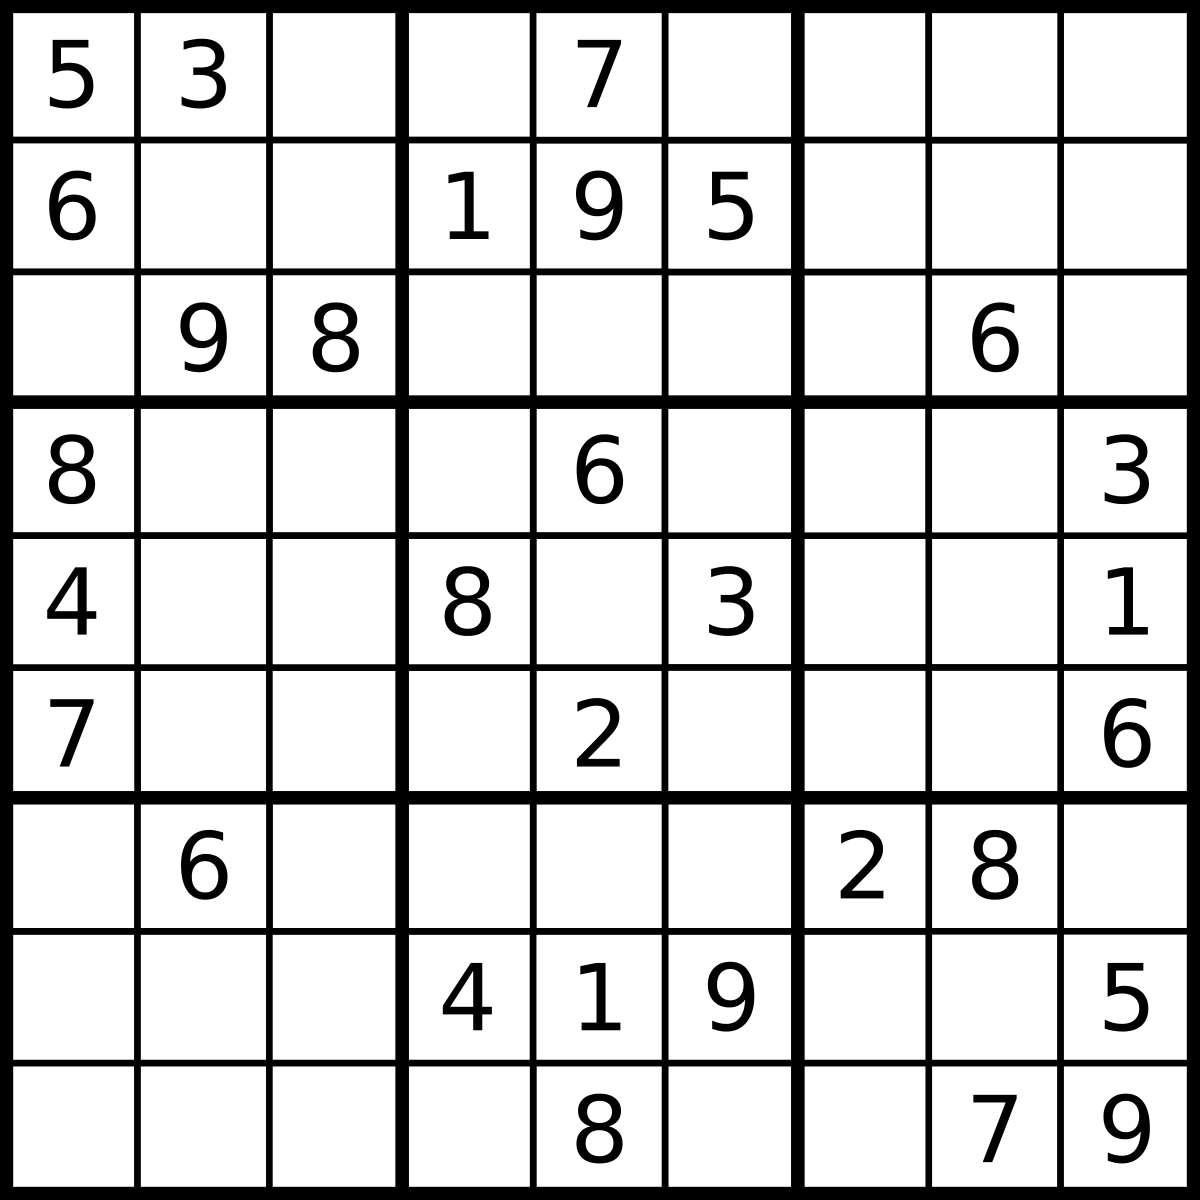
\includegraphics[scale=0.12]{./figures/classicSUDOKU.jpeg}
		\caption{\el Παράδειγμα κλασσικού \textbf{\en Sudoku} \(9 \times 9\)}
	\end{figure}
\end{frame}

\begin{frame}
	\frametitle{\el Εισαγωγή}
	\begin{itemize}
		\item \el Στόχος του παιχνιδιού είναι ο παίκτης να συμπληρώσει τα κενά κελιά ενός ημιτελώς συμπληρωμένου πίνακα.
	\end{itemize}
\end{frame}

\begin{frame}
	\frametitle{\el Εισαγωγή}
	\begin{mytheorem}{\textbf{\en Sudoku}}{}
		\el Οι κανόνες για το κλασσικό \textbf{\en Sudoku} \el σε έναν πίνακα μεγέθους \(n \times n\) με υποπίνακες μεγέθους \(m \times m\), 	όπου \(m = \sqrt{n}\) είναι: \\
		\(\bullet\)\el Κάθε γραμμή του πίνακα μεγέθους \en n \el να περιέχει ακριβώς μια φορά κάθε ακέραιο αριθμό από το 1 ως το \en n. \\
		\(\bullet\)\el Κάθε στήλη του πίνακα μεγέθους \en n \el να περιέχει ακριβώς μια φορά κάθε ακέραιο αριθμό από το 1 ως το \en n. \\
		\(\bullet\)\el Κάθε υποπίνακας μεγέθους \(m \times m\) να περιέχει ακριβώς μια φορά κάθε ακέραιο αριθμό από το 1 ως το \en n. \\
	\end{mytheorem}
\end{frame}

\begin{frame}
	\frametitle{\el Εισαγωγή}
	\begin{itemize}
		\item \el Οι αριθμοί μπορούν να αντικατασταθούν με οποιαδήποτε ομάδα συμβόλων, χωρίς να προκαλέσουν καμμία επίπτωση στην
		      επίλυση, στη δημιουργία ή στη μαθηματική μοντελοποίηση του παζλ.
		\item \el Υπάρχουν διαθέσιμα \en
		      \textbf{Sudoku} \el παζλ με βάση κινέζικα σύμβολα, κινέζικους αριθμούς και σύμβολα που αναπαριστούν
		      μερίδες σούσι.
	\end{itemize}
\end{frame}

\begin{frame}
	\frametitle{\el Ιστορία}
	\begin{itemize}
		\item \el Δημιουργός του εν λόγω παιχνιδιού υπήρξε ο Αμερικανός αρχιτέκτονας \en Howard Garns \el (Μάρτιος 1905 - Οκτώβριος 1989) το 1979.
		\item Το παιχνίδι αρχικά ονομάστηκε \en “Number Place” \el και δημοσιεύτηκε στο περιοδικό \en Dell Pencil Puzzles \& Word Games.
		\item \el Ένα χρόνο μετά το παιχνίδι έγινε ιδιαίτερα δημοφιλές στην Ιαπωνία και μετονομάστηκε σε \en “suji wa dokushin ni kagiru”(\textbf{Sudoku}).
	\end{itemize}
	\begin{figure}
		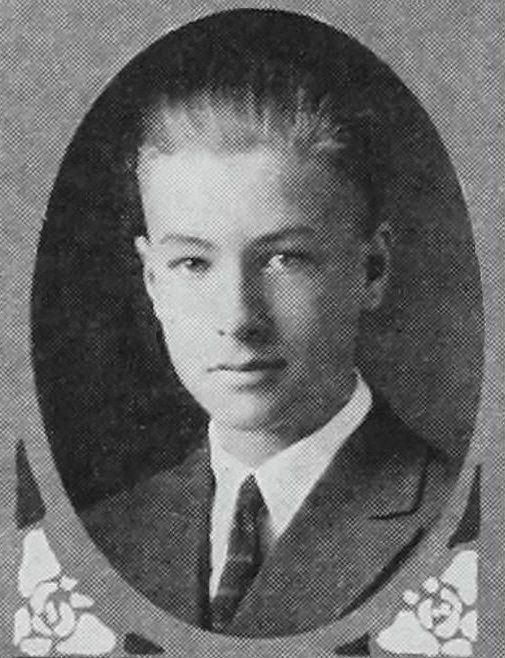
\includegraphics[scale=0.1]{./figures/Howard Garns.jpeg}
		\caption{Howard Garns}
	\end{figure}
\end{frame}

\begin{frame}
	\frametitle{\el Ιστορία}
	\begin{itemize}
		\item \el Το \textbf{\en Sudoku} \el έγινε ιδιαίτερα αγαπητό στην Ιαπωνία, με τις μηνιαίες πωλήσεις \textbf{\en Sudoku} \el περιοδικών να ανέρχονται στα 600.000 αντίτυπα κάθε μήνα.
		\item Οι Ιάπωνες υιοθέτησαν το \textbf{\en Sudoku} \el ως συνήθεια για δύο βασικούς λόγους:
		      \begin{itemize}
			      \item η γλώσσα τους δεν ήταν κατάλληλη για την ανάπτυξη σταυρόλεξων, οπότε υστερούσαν σε αυτά και
			      \item συνηθίζουν να μετακινούνται με τρένα και λεωφορεία.
		      \end{itemize}
	\end{itemize}
\end{frame}

\begin{frame}
	\frametitle{\el Ιστορία}
	\begin{figure}
		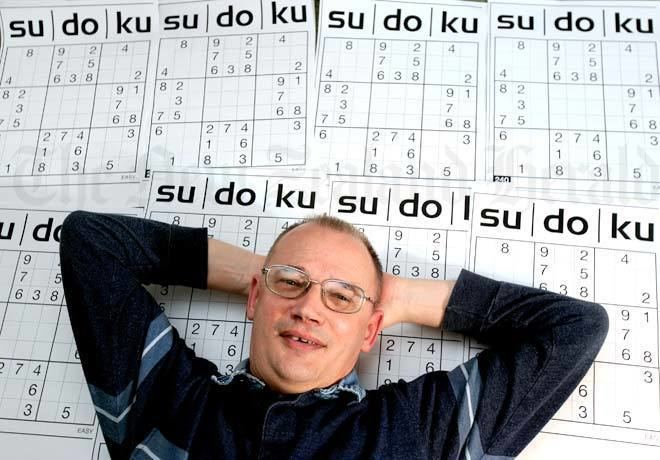
\includegraphics[scale=0.2]{./figures/WayneGould.jpg}
		\caption{Wayne Gould}
	\end{figure}
	\begin{itemize}
		\item \el Ο \en Wayne Gould \el, Νεοζηλανδός δικαστής, έφερε πίσω στον Δυτικό κόσμο το \textbf{\en Sudoku}.
		\item \el To 1997 βρισκόταν στο Τόκιο και ανακάλυψε ενα \textbf{\en Sudoku}.
		\item \el Έφτιαξε το πρωτο πρόγραμμα που δημιουργούσε \textbf{\en Sudoku} \el παζλ.
	\end{itemize}
\end{frame}

\begin{frame}
	\frametitle{\el Μελέτη}
	\el Στην παρούσα εργασία θα μελετήσουμε σε βάθος: \\

	\begin{itemize}
		\item \el Μαθηματικές μεθοδολογίες για την επίλυση \en sudoku.
		      \begin{itemize}
			      \item \el Μοντελοποίηση του προβλήματος της επίλυσης του παζλ ως πρόβλημα γραμμικού προγραμματισμού.
			      \item \el Παραλλαγές του κλασσικού \en sudoku.
			      \item Υλοποίηση σε \textbf{\en python}.
		      \end{itemize}
		\item \el Μαθηματικές τεχνικές για τη δημιουργία \en sudoku.
		      \begin{itemize}
			      \item \el Κριτήρια \en sudoku \el παζλ.
			      \item \el Δημιουργία \en sudoku \el με \en bruteforce.
			      \item \el Δημιουργία \en sudoku \el από προγενέστερο παζλ.
			      \item \el Δημουργία \textbf{\en Sudoku} \el παζλ βάση λογικών στρατηγικών.
			      \item Υλοποίηση σε \textbf{\en python}.
		      \end{itemize}
		\item \el Επίπεδα δυσκολίας \textbf{\en Sudoku} \el παζλ
		      \begin{itemize}
			      \item \el Μελέτη των επιπέδων δυσκολίας στην επίλυση \textbf{\en Sudoku} \el παζλ από τον άνθρωπο
			      \item \el Στατιστική προσέγγιση
			      \item \el Επίπεδο δυσκολίας και δεδομένοι όροι στο παζλ.
		      \end{itemize}
	\end{itemize}
\end{frame}

\begin{frame}
	\frametitle{\el Μαθηματική μοντελοποίηση}
	\begin{itemize}
		\item \el Η μαθηματική μοντελοποίηση καθιστά δυνατή την εύρεση της λύσης του παζλ, αν υπάρχει, από
		      έναν μαθηματικό αλγόριθμο.
		\item \el Το πρόβλημα επίλυσης ενός \textbf{\en Sudoku} \el παζλ είναι πρόβλημα ικανοποίησης περιορισμών.
	\end{itemize}
\end{frame}

\begin{frame}
	\frametitle{\el Μαθηματική μοντελοποίηση}
	\begin{itemize}
		\item \el Ένα πρόβλημα ικανοποίησης περιορισμών ορίζεται από δύο σύνολα:
		      \begin{itemize}
			      \item \el το σύνολο μεταβλητών, \(X_1, X_2, \dots, X_t\),
			      \item \el το σύνολο περιορισμών, \(C_1, C_2, \dots, C_z\)
		      \end{itemize}
		\item \el Κάθε μεταβλητή \(X_i\) με \(1 \leq i \leq t\) λαμβάνει τιμές από ένα πεδίο \(D_i\).
		\item Κάθε περιορισμός \(C_j\) με \(1 \leq j \leq z\) αφορά κάποιο υποσύνολο των μεταβλητών και καθορίζει ποιος είναι ο επιτρεπτός συνδυασμός τιμών για αυτό το υποσύνολο μεταβλητών.
	\end{itemize}
\end{frame}

\begin{frame}
	\frametitle{\el Μαθηματική μοντελοποίηση}
	\begin{itemize}
		\item \el Έστω, ο \(n \times n\) πίνακας \textbf{\en Sudoku} \el και οι υποπίνακες του μεγέθους \(m \times m\).
		\item \el Ορίζουμε τις μεταβλητές απόφασης ως εξής:
		      \[
			      x_{ijk} =
			      \begin{cases}
				      1 & \quad\text{αν το κελι \en (i,j) \el του πίνακα περιέχει τον ακέραιο \en k} \\
				      0 & \quad\text{\el αλλιώς}                                                     \\
			      \end{cases}
		      \]
	\end{itemize}
\end{frame}

\begin{frame}
	\frametitle{\el Μαθηματική μοντελοποίηση}
	\begin{itemize}
		\item \el Η μοντελοποίηση του προβλήματος είναι:
	\end{itemize}
	\begin{align*}
		\min \quad 0^{T}x \\
		\begin{aligned}
			\textup{\en s.t.}\quad
			\sum_{i=1}^{n}x_{ijk} = 1 \quad j=1:n, \quad k=1:n \\ \textit{\el μόνο ένα \en k \el σε κάθε στήλη του πίνακα} \\
			\sum_{j=1}^{n}x_{ijk} = 1 \quad i=1:n, \quad k=1:n \\ \text{\el μόνο ένα \en k \el σε κάθε γραμμή του πίνακα} \\
		\end{aligned}
	\end{align*}
\end{frame}

\begin{frame}
	\frametitle{\el Μαθηματική μοντελοποίηση}
	\begin{align*}
		\begin{aligned}
			\sum_{j=mq-m+1}^{mq} {\sum_{i=mp-m+1}^{mp}x_{ijk}} = 1 \quad k=1:n, \quad p=1:m, \quad q=1:m \\ \text{\el μόνο ένας ακέραιος \en k \el σε κάθε υποπίνακα} \\
			\sum_{k=1}^{n}x_{ijk} = 1 \quad i=1:n, \quad j=1:n                                           \\ \text{\el όλα τα κελιά του πίνακα πρέπει να συμπληρωθούν} \\
			x_{ijk} = 1 \forall (i,j,k) \in G                                                            \\ \text{\el τα κελιά του πίνακα που είναι συμπληρωμένα είναι \en "on"} \\
			x_{ijk} \in {0,1}
		\end{aligned}
	\end{align*}
\end{frame}

\begin{frame}
	\frametitle{\el Παραλλαγές}
	\begin{itemize}
		\item \el Υπάρχουν παραλλαγές του κλασσικού παζλ \textbf{\en Sudoku},
		\item \el Η επίλυσή τους είναι πιο απαιτητική σε σχέση με το κλασσικό παζλ.
		\item \el Η μοντελοποίησή του δε διαφέρει
		      ιδιαίτερα από τη μοντελοποίηση για τα κλασσικά παζλ \textbf{\en Sudoku}.
	\end{itemize}
\end{frame}

\begin{frame}
	\frametitle{\textbf{\en Sudoku} X}
	\begin{itemize}
		\item \el Το \textbf{\en Sudoku} X \el είναι μία παραλλαγή του κλασσικού \textbf{\en Sudoku}.
		\item \el Έχει τον επιπλεόν κανόνα ότι οι δύο μεγάλες διαγώνιοι του πίνακα πρέπει να περιέχουν κάθε ψηφίο από το 1 μέχρι το \en n \el ακριβώς μία φορά η κάθε μία.
	\end{itemize}
\end{frame}

\begin{frame}
	\frametitle{\textbf{\en Sudoku} X}
	\begin{figure}[h]
		\centering
		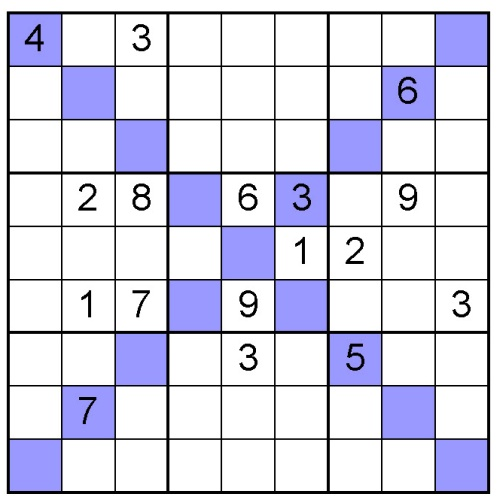
\includegraphics[scale=0.7]{figures/sudokuX.jpg}
		\caption{Παράδειγμα ενός \textbf{Sudoku} X παζλ. Οι δύο μεγάλες διαγώνιοι είναι σημειωμένες με μωβ χρώμα. Η κάθε μία πρέπει να περιέχει όλους τους αριθμούς από το 1 εως και το 9 ακριβώς μία φορα τον καθέναν.}
	\end{figure}
\end{frame}

\begin{frame}
	\frametitle{\textbf{\en Sudoku} X}
	\begin{mytheorem}{\textbf{\en Sudoku} X}{}
		\el Οι κανόνες για το \textbf{\en Sudoku} X \el σε έναν πίνακα μεγέθους \(n \times n\) με υποπίνακες μεγέθους \(m \times m\), όπου \(m = \sqrt{n}\) είναι: \\
		\(\bullet\) \el Κάθε γραμμή του πίνακα μεγέθους \en n \el να περιέχει ακριβώς μια φορά κάθε ακέραιο αριθμό από το 1 ως το \en n. \\
		\(\bullet\) \el Κάθε στήλη του πίνακα μεγέθους \en n \el να περιέχει ακριβώς μια φορά κάθε ακέραιο αριθμό από το 1 ως το \en n. \\
		\(\bullet\) \el Κάθε υποπίνακας μεγέθους \(m \times m\) να περιέχει ακριβώς μια φορά κάθε ακέραιο αριθμό από το 1 ως το \en n. \\
		\(\bullet\) \el Η διαγώνιος του πίνακα που ξεκινά από το κελί (1,1) και καταλήγει στο κελί \en (n,n) \el να περιέχει ακριβώς μια φορά κάθε ακέραιο αριθμό από το 1 ως το \en n. \\
		\(\bullet\) \el Η διαγώνιος του πίνακα που ξεκινά από το κελί \en (1,n) \el και καταλήγει στο κελί \en (n,1) \el να περιέχει ακριβώς μια φορά κάθε ακέραιο αριθμό από το 1 ως το \en n. \\

	\end{mytheorem}
\end{frame}

\begin{frame}
	\frametitle{\textbf{\en Sudoku} X}
	\begin{itemize}
		\item \el Η μοντελοποίηση του προβλήματος είναι:
	\end{itemize}
	\begin{align*}
		\min \quad 0^{T}x \\
		\begin{aligned}
			\textup{\en s.t.}\quad
			\sum_{i=1}^{n}x_{ijk} = 1 \quad j=1:n, \quad k=1:n \\ \textit{\el μόνο ένα \en k \el σε κάθε στήλη του πίνακα} \\
			\sum_{j=1}^{n}x_{ijk} = 1 \quad i=1:n, \quad k=1:n \\ \text{\el μόνο ένα \en k \el σε κάθε γραμμή του πίνακα} \\
		\end{aligned}
	\end{align*}
\end{frame}

\begin{frame}
	\frametitle{\textbf{\en Sudoku} X}
	\begin{align*}
		\begin{aligned}
			\sum_{j=mq-m+1}^{mq} {\sum_{i=mp-m+1}^{mp}x_{ijk}} = 1 \quad k=1:n, \quad p=1:m, \quad q=1:m \\ \text{\el μόνο ένας ακέραιος \en k \el σε κάθε υποπίνακα} \\
			\sum_{r=1}^{n} x_{rrk} = 1 \quad k=1:9                                                       \\ \text{\el μόνο ένα \en k \el στην κύρια διαγώνιο} \\
			\sum_{r=1}^{n} x_{r(n+1-r)k} = 1 \quad k=1:9                                                 \\ \text{\el μόνο ένα \en k \el στη δευτερεύουσα διαγώνιο} \\
		\end{aligned}
	\end{align*}
\end{frame}


\begin{frame}
	\frametitle{\textbf{\en Sudoku} X}
	\begin{align*}
		\begin{aligned}
			\sum_{k=1}^{n}x_{ijk} = 1 \quad i=1:n, \quad j=1:n \\ \text{\el όλα τα κελιά του πίνακα πρέπει να συμπληρωθούν} \\
			x_{ijk} = 1 \forall (i,j,k) \in G                  \\ \text{\el τα κελιά του πίνακα που είναι συμπληρωμένα είναι \en "on"} \\
			x_{ijk} \in {0,1}
		\end{aligned}
	\end{align*}
\end{frame}

\begin{frame}
	\frametitle{\en Four Square \textbf{Sudoku}}
	\begin{itemize}
		\item \el Το \en Four Square \textbf{Sudoku} \el είναι μία παραλλαγή του κλασσικού \textbf{\en Sudoku}.
		\item \el Υποθέτουμε ότι αναφερόμαστε σε παζλ \(9 \times 9\).
		\item \el Ο επιπλεόν κανόνας εδώ σχετίζεται με τέσσερις επιπλέον υποπεριοχές στον πίνακα μεγέθους \(3 \times 3\). Στίς περιοχές αυτες πρέπει να περιέχονται όλοι οι ακέραιοι αριθμοί από το 1 ως το 9.
	\end{itemize}
\end{frame}

\begin{frame}
	\frametitle{\en Four Square \textbf{Sudoku}}
	\begin{figure}[h]
		\centering
		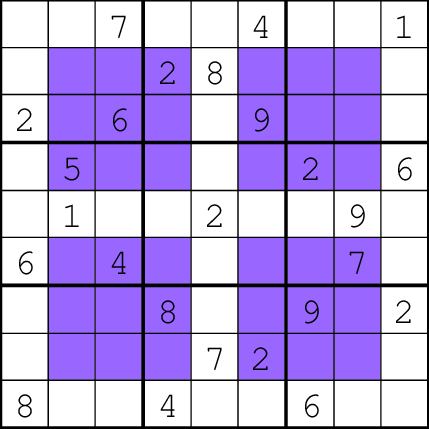
\includegraphics[scale=0.4]{figures/An-example-Four-Square-Sudoku-puzzle.png}
		\caption{Παράδειγμα ενός Four Square \textbf{Sudoku} παζλ. Οι τέσσερις περιοχές είναι σημειωμένες με μωβ χρώμα. Η κάθε μία πρέπει να περιέχει όλους τους αριθμούς από το 1 εως και το 9 ακριβώς μία φορα τον καθέναν.}
	\end{figure}
\end{frame}

\begin{frame}
	\frametitle{\en Four Square \textbf{Sudoku}}
	\begin{mytheorem}{\en Four Square \textbf{Sudoku}}{}
		Οι κανόνες για το Four Square \textbf{Sudoku} σε έναν πίνακα μεγέθους \(9 \times 9\) με υποπίνακες μεγέθους \(3 \times 3\) είναι: \\
		\(\bullet\) Κάθε γραμμή του πίνακα μεγέθους 9 να περιέχει ακριβώς μια φορά κάθε ακέραιο αριθμό από το 1 ως το n. \\
		\(\bullet\) Κάθε στήλη του πίνακα μεγέθους 9 να περιέχει ακριβώς μια φορά κάθε ακέραιο αριθμό από το 1 ως το 9. \\
		\(\bullet\) Κάθε υποπίνακας μεγέθους \(3 \times 3\) να περιέχει ακριβώς μια φορά κάθε ακέραιο αριθμό από το 1 ως το 9. \\
		\(\bullet\) Κάθε υποπεριοχή μεγέθους
		\(3 \times 3\) να περιέχει όλους τους ακέραιους από το 1 ως το 9. \\
	\end{mytheorem}
\end{frame}

\begin{frame}
	\frametitle{\en Four Square \textbf{Sudoku}}
	\begin{itemize}
		\item \el Η μοντελοποίηση του προβλήματος είναι:
	\end{itemize}
	\begin{align*}
		\min \quad 0^{T}x \\
		\begin{aligned}
			\textup{\en s.t.}\quad
			\sum_{i=1}^{n}x_{ijk} = 1 \quad j=1:n, \quad k=1:n \\ \textit{\el μόνο ένα \en k \el σε κάθε στήλη του πίνακα} \\
			\sum_{j=1}^{n}x_{ijk} = 1 \quad i=1:n, \quad k=1:n \\ \text{\el μόνο ένα \en k \el σε κάθε γραμμή του πίνακα} \\
		\end{aligned}
	\end{align*}
\end{frame}

\begin{frame}
	\frametitle{\en Four Square \textbf{Sudoku}}
	\begin{align*}
		\begin{aligned}
			\sum_{j=mq-m+1}^{mq} {\sum_{i=mp-m+1}^{mp}x_{ijk}} = 1 \quad k=1:n, \quad p=1:m, \quad q=1:m \\ \text{\el μόνο ένας ακέραιος \en k \el σε κάθε υποπίνακα} \\
			\sum_{r=i}^{i+2}{\sum_{c=j}^{j+2}x_{rck}} = 1 \quad i=2,6; \quad j=2,6; \quad k=1:9          \\ \text{\el μόνο ένας ακέραιος \en k \el σε κάθε υποπεριοχή} \\
		\end{aligned}
	\end{align*}
\end{frame}

\begin{frame}
	\frametitle{\en Four Square \textbf{Sudoku}}
	\begin{align*}
		\begin{aligned}
			\sum_{k=1}^{n}x_{ijk} = 1 \quad i=1:n, \quad j=1:n \\ \text{\el όλα τα κελιά του πίνακα πρέπει να συμπληρωθούν} \\
			x_{ijk} = 1 \forall (i,j,k) \in G                  \\ \text{\el τα κελιά του πίνακα που είναι συμπληρωμένα είναι \en "on"} \\
			x_{ijk} \in {0,1}
		\end{aligned}
	\end{align*}
\end{frame}

\begin{frame}
	\frametitle{\en Four Pyramids \textbf{Sudoku}}
	\begin{itemize}
		\item \el Το \en Four Pyramids \textbf{Sudoku} \el είναι μία παραλλαγή του κλασσικού \textbf{\en Sudoku}.
		\item \el Υποθέτουμε ότι αναφερόμαστε σε παζλ \(9 \times 9\).
		\item \el Η παραλλαγή είναι παρόμοια με την παραλλαγή στο \en Four Square \textbf{Sudoku} \el , με τη διαφορά ότι εδώ οι επιπλέον υποπεριοχές του πίνακα έχουν τριγωνική μορφή.
	\end{itemize}
\end{frame}

\begin{frame}
	\frametitle{\en Four Pyramids \textbf{Sudoku}}
	\begin{figure}[h]
		\centering
		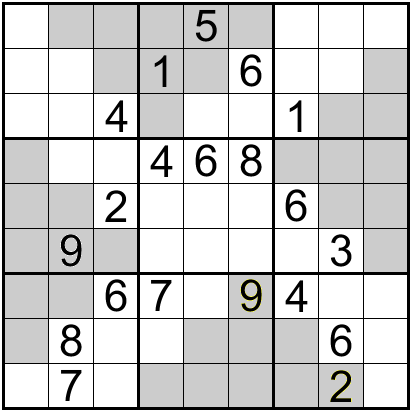
\includegraphics[scale=0.4]{figures/Pyramid Sudoku.png}
		\caption{Παράδειγμα ενός Four Pyramids \textbf{Sudoku} παζλ. Οι τέσσερις τριγωνικές περιοχές είναι σημειωμένες με γκρί χρώμα. Η κάθε μία πρέπει να περιέχει όλους τους αριθμούς από το 1 εως και το 9 ακριβώς μία φορα τον καθέναν.}
	\end{figure}
\end{frame}

\begin{frame}
	\frametitle{\en Four Pyramids \textbf{Sudoku}}
	\begin{mytheorem}{\en Four Pyramids \textbf{Sudoku}}{}
		Οι κανόνες για το Four Pyramids \textbf{Sudoku} σε έναν πίνακα μεγέθους \(9 \times 9\) με υποπίνακες μεγέθους \(3 \times 3\) είναι: \\
		\(\bullet\) Κάθε γραμμή του πίνακα μεγέθους 9 να περιέχει ακριβώς μια φορά κάθε ακέραιο αριθμό από το 1 ως το n. \\
		\(\bullet\) Κάθε στήλη του πίνακα μεγέθους 9 να περιέχει ακριβώς μια φορά κάθε ακέραιο αριθμό από το 1 ως το 9. \\
		\(\bullet\) Κάθε υποπίνακας μεγέθους \(3 \times 3\) να περιέχει ακριβώς μια φορά κάθε ακέραιο αριθμό από το 1 ως το 9. \\
		\(\bullet\) Κάθε υποπεριοχή μεγέθους
		\(3 \times 3\) να περιέχει όλους τους ακέραιους από το 1 ως το 9. \\
	\end{mytheorem}
\end{frame}

\begin{frame}
	\frametitle{\en Four Pyramids \textbf{Sudoku}}
	\begin{itemize}
		\item \el Η μοντελοποίηση του προβλήματος είναι:
	\end{itemize}
	\begin{align*}
		\min \quad 0^{T}x \\
		\begin{aligned}
			\textup{\en s.t.}\quad
			\sum_{i=1}^{n}x_{ijk} = 1 \quad j=1:n, \quad k=1:n \\ \textit{\el μόνο ένα \en k \el σε κάθε στήλη του πίνακα} \\
			\sum_{j=1}^{n}x_{ijk} = 1 \quad i=1:n, \quad k=1:n \\ \text{\el μόνο ένα \en k \el σε κάθε γραμμή του πίνακα} \\
		\end{aligned}
	\end{align*}
\end{frame}

\begin{frame}
	\frametitle{\en Four Pyramids \textbf{Sudoku}}
	\begin{align*}
		\begin{aligned}
			\sum_{j=mq-m+1}^{mq} {\sum_{i=mp-m+1}^{mp}x_{ijk}} = 1 \quad k=1:n, \quad p=1:m, \quad q=1:m \\ \text{\el μόνο ένας ακέραιος \en k \el σε κάθε υποπίνακα} \\
		\end{aligned}
	\end{align*}
\end{frame}

\begin{frame}
	\frametitle{\en Four Pyramids \textbf{Sudoku}}
	\begin{align*}
		\begin{aligned}
			\sum_{r=1}^{3}{\sum_{c=3+r}^{9-r} x_{rck}} = 1 \quad k=1:9  \\ \text{\el η πρώτη πυραμίδα να έχει μόνο ένα \en k} \\
			\sum_{c=1}^{3}{\sum_{r=1+c}^{7-c} x_{rck}} = 1 \quad k=1:9  \\ \text{\el η δεύτερη πυραμίδα να έχει μόνο ένα \en k}\\
			\sum_{r=7}^{9}{\sum_{c=11-r}^{r-7} x_{rck}} = 1 \quad k=1:9 \\ \text{\el η τρίτη πυραμίδα να έχει μόνο ένα \en k} \\
			\sum_{c=7}^{9}{\sum_{r=13-c}^{c-1} x_{rck}} = 1 \quad k=1:9 \\ \text{\el η τέταρτη πυραμίδα να έχει μόνο ένα \en k} \\
		\end{aligned}
	\end{align*}
\end{frame}

\begin{frame}
	\frametitle{\en Four Pyramids \textbf{Sudoku}}
	\begin{align*}
		\begin{aligned}
			\sum_{k=1}^{n}x_{ijk} = 1 \quad i=1:n, \quad j=1:n \\ \text{\el όλα τα κελιά του πίνακα πρέπει να συμπληρωθούν} \\
			x_{ijk} = 1 \forall (i,j,k) \in G                  \\ \text{\el τα κελιά του πίνακα που είναι συμπληρωμένα είναι \en "on"} \\
			x_{ijk} \in {0,1}
		\end{aligned}
	\end{align*}
\end{frame}

\begin{frame}
	\frametitle{\en Position \textbf{Sudoku}}
	\begin{itemize}
		\item \el Το \en Position \textbf{Sudoku} \el είναι μία παραλλαγή του κλασσικού \textbf{\en Sudoku}.
		\item \el Υποθέτουμε ότι αναφερόμαστε σε παζλ \(9 \times 9\).
		\item \el Τα κελιά (1,1) σε όλους τους \(3 \times 3\) υποπίνακες πρέπει να περιέχουν όλους τους ακέραιους από το 1 ως το 9 ακριβώς μια φορά, αντίστοιχα τα κελιά (1,2) όλων των υποπινάκων κοκ.
	\end{itemize}
\end{frame}

\begin{frame}
	\frametitle{\en Position \textbf{Sudoku}}
	\begin{figure}[h]
		\centering
		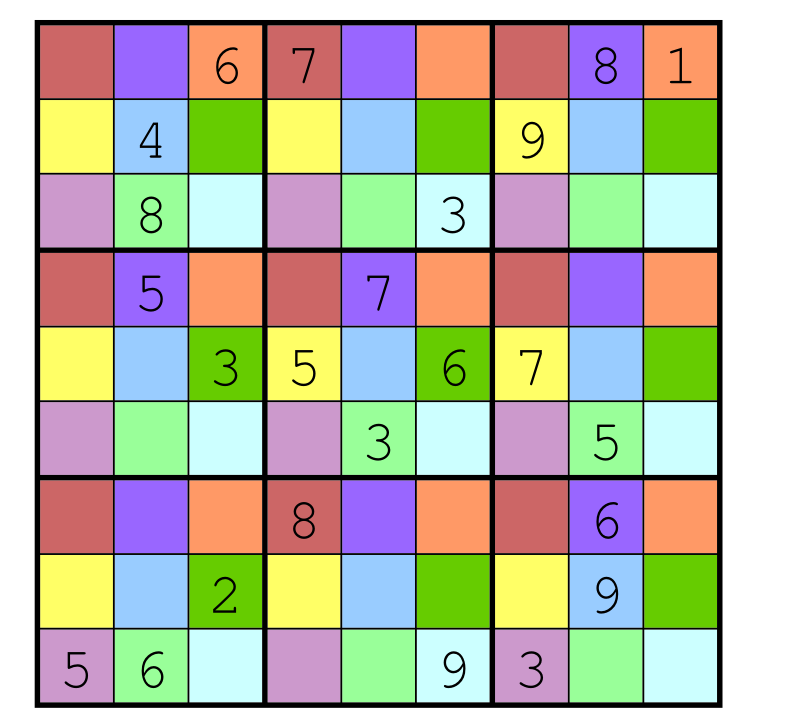
\includegraphics[scale=0.2]{figures/positionSUDOKU.png}
		\caption{Παράδειγμα ενός Position \textbf{Sudoku} παζλ. Κάθε κελί με το ίδιο χρώμα πρέπει να περιέχει όλους τους αριθμούς από το 1 εως και το 9 ακριβώς μία φορα τον καθέναν.}
	\end{figure}
\end{frame}

\begin{frame}
	\frametitle{\en Position \textbf{Sudoku}}
	\begin{mytheorem}{\en Position \textbf{Sudoku}}{}
		Οι κανόνες για το Position \textbf{Sudoku} σε έναν πίνακα μεγέθους \(9 \times 9\) με υποπίνακες μεγέθους \(3 \times 3\) είναι: \\
		\(\bullet\) Κάθε γραμμή του πίνακα μεγέθους 9 να περιέχει ακριβώς μια φορά κάθε ακέραιο αριθμό από το 1 ως το n. \\
		\(\bullet\) Κάθε στήλη του πίνακα μεγέθους 9 να περιέχει ακριβώς μια φορά κάθε ακέραιο αριθμό από το 1 ως το 9. \\
		\(\bullet\) Κάθε υποπίνακας μεγέθους \(3 \times 3\) να περιέχει ακριβώς μια φορά κάθε ακέραιο αριθμό από το 1 ως το 9. \\
		\(\bullet\) Κάθε κελί (i,j) με i=1:9 και j=1:9 σε όλους τους υποπίνακες \(3 \times 3\) να περιέχει ακριβώς μια φορά κάθε ακέραιο αριθμό από το 1 ως το 9.
	\end{mytheorem}
\end{frame}

\begin{frame}
	\frametitle{\en Position \textbf{Sudoku}}
	\begin{itemize}
		\item \el Η μοντελοποίηση του προβλήματος είναι:
	\end{itemize}
	\begin{align*}
		\min \quad 0^{T}x \\
		\begin{aligned}
			\textup{\en s.t.}\quad
			\sum_{i=1}^{n}x_{ijk} = 1 \quad j=1:n, \quad k=1:n \\ \textit{\el μόνο ένα \en k \el σε κάθε στήλη του πίνακα} \\
			\sum_{j=1}^{n}x_{ijk} = 1 \quad i=1:n, \quad k=1:n \\ \text{\el μόνο ένα \en k \el σε κάθε γραμμή του πίνακα} \\
		\end{aligned}
	\end{align*}
\end{frame}

\begin{frame}
	\frametitle{\en Position \textbf{Sudoku}}
	\begin{align*}
		\begin{aligned}
			\sum_{j=mq-m+1}^{mq} {\sum_{i=mp-m+1}^{mp}x_{ijk}} = 1 \quad k=1:n, \quad p=1:m, \quad q=1:m \\ \text{\el μόνο ένας ακέραιος \en k \el σε κάθε υποπίνακα} \\
			\sum_{i=c}^{9}{\sum_{j=z}^{9} x_{ijk}} = 1 \quad c=1:(3):9 \quad j=1:(3):9 \quad k=1:9       \\ \text{μόνο ένα k σε κελιά υποπινάκων με ίδιες συντεταγμένες } \\
		\end{aligned}
	\end{align*}
\end{frame}

\begin{frame}
	\frametitle{\en Position \textbf{Sudoku}}
	\begin{align*}
		\begin{aligned}
			\sum_{k=1}^{n}x_{ijk} = 1 \quad i=1:n, \quad j=1:n \\ \text{\el όλα τα κελιά του πίνακα πρέπει να συμπληρωθούν} \\
			x_{ijk} = 1 \forall (i,j,k) \in G                  \\ \text{\el τα κελιά του πίνακα που είναι συμπληρωμένα είναι \en "on"} \\
			x_{ijk} \in {0,1}
		\end{aligned}
	\end{align*}
\end{frame}

\begin{frame}
	\frametitle{\en Three Magic \textbf{Sudoku}}
	\begin{itemize}
		\item \el Το \en Three Magic \textbf{Sudoku} \el είναι μία παραλλαγή του κλασσικού \textbf{\en Sudoku}.
		\item \el Υποθέτουμε ότι αναφερόμαστε σε παζλ \(9 \times 9\).
		\item \el Στα σημειωμένα \(3 \times 3\) κουτιά \en (magic) \el οι 3 αριθμοί σε κάθε στήλη και οι 3 αριθμοί σε κάθε γραμμή αν αθροιστούν δίνουν το ίδιο αποτέλεσμα.
	\end{itemize}
\end{frame}

\begin{frame}
	\frametitle{\en Three Magic \textbf{Sudoku}}
	\begin{figure}[h]
		\centering
		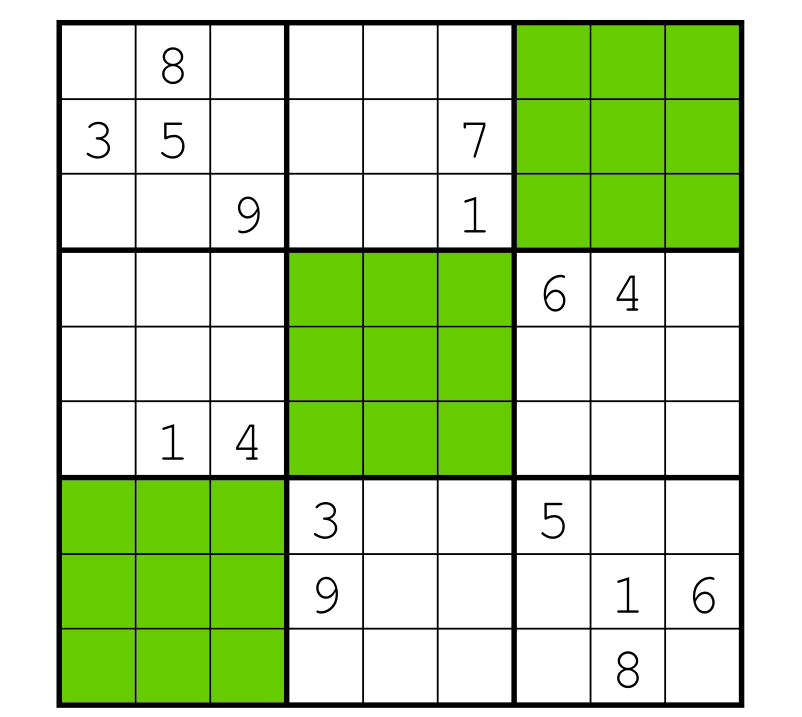
\includegraphics[scale=0.2]{figures/threemagicSUDOKU.png}
		\caption{Παράδειγμα ενός Three Magic \textbf{Sudoku} παζλ. Οι 3 αριθμοί σε κάθε στήλη και οι 3 αριθμοί σε κάθε γραμμή στα πράσινα \(3 \times 3\) κουτιά πρέπει αν προτεθούν να δίνουν τον ίδιο αριθμό.}
	\end{figure}
\end{frame}

\begin{frame}
	\frametitle{\en Three Magic \textbf{Sudoku}}
	\begin{mytheorem}{\en Three Magic \textbf{Sudoku}}{}
		Οι κανόνες για το Three Magic \textbf{Sudoku} σε έναν πίνακα μεγέθους \(9 \times 9\) με υποπίνακες μεγέθους \(3 \times 3\) είναι: \\
		\(\bullet\) Κάθε γραμμή του πίνακα μεγέθους 9 να περιέχει ακριβώς μια φορά κάθε ακέραιο αριθμό από το 1 ως το n. \\
		\(\bullet\) Κάθε στήλη του πίνακα μεγέθους 9 να περιέχει ακριβώς μια φορά κάθε ακέραιο αριθμό από το 1 ως το 9. \\
		\(\bullet\) Κάθε υποπίνακας μεγέθους \(3 \times 3\) να περιέχει ακριβώς μια φορά κάθε ακέραιο αριθμό από το 1 ως το 9. \\
		\(\bullet\) Σε κάθε μαγικό κουτί το άθροισμα των στηλών και των γραμμών πρέπει να είναι το ίδιο.
	\end{mytheorem}
\end{frame}

\begin{frame}
	\frametitle{\en Three Magic \textbf{Sudoku}}
	\begin{itemize}
		\item \el Η μοντελοποίηση του προβλήματος είναι:
	\end{itemize}
	\begin{align*}
		\min \quad 0^{T}x \\
		\begin{aligned}
			\textup{\en s.t.}\quad
			\sum_{i=1}^{n}x_{ijk} = 1 \quad j=1:n, \quad k=1:n \\ \textit{\el μόνο ένα \en k \el σε κάθε στήλη του πίνακα} \\
			\sum_{j=1}^{n}x_{ijk} = 1 \quad i=1:n, \quad k=1:n \\ \text{\el μόνο ένα \en k \el σε κάθε γραμμή του πίνακα} \\
		\end{aligned}
	\end{align*}
\end{frame}

\begin{frame}
	\frametitle{\en Three Magic \textbf{Sudoku}}
	\begin{align*}
		\begin{aligned}
			\sum_{j=mq-m+1}^{mq} {\sum_{i=mp-m+1}^{mp}x_{ijk}} = 1 \quad k=1:n, \quad p=1:m, \quad q=1:m \\ \text{\el μόνο ένας ακέραιος \en k \el σε κάθε υποπίνακα} \\
			............................................
		\end{aligned}
	\end{align*}
\end{frame}

\begin{frame}
	\frametitle{\en Three Magic \textbf{Sudoku}}
	\begin{align*}
		\begin{aligned}
			\sum_{k=1}^{n}x_{ijk} = 1 \quad i=1:n, \quad j=1:n \\ \text{\el όλα τα κελιά του πίνακα πρέπει να συμπληρωθούν} \\
			x_{ijk} = 1 \forall (i,j,k) \in G                  \\ \text{\el τα κελιά του πίνακα που είναι συμπληρωμένα είναι \en "on"} \\
			x_{ijk} \in {0,1}
		\end{aligned}
	\end{align*}
\end{frame}

\begin{frame}
	\frametitle{\el Δημιουργία \textbf{\en Sudoku} \el παζλ}
	\begin{itemize}
		\item \el Κριτήρια \en sudoku \el παζλ.
		\item \el Δημιουργία \en sudoku \el με \en bruteforce.
		\item \el Δημιουργία \en sudoku \el από προγενέστερο παζλ.
		\item \el Δημουργία \textbf{\en Sudoku} \el παζλ βάση λογικών στρατηγικών .
	\end{itemize}
\end{frame}

\begin{frame}
	\frametitle{\el Κριτήρια \textbf{\en Sudoku} \el παζλ}
	\begin{itemize}
		\item \el Ενα παζλ \textbf{\en Sudoku} \el οφείλει να πληρεί ορισμένες βασικές προϋποθέσεις,
		      \begin{itemize}
			      \item \el για να έχει λύση
			      \item \el για να επιθυμεί κάποιος να ενασχοληθεί με αυτό.
		      \end{itemize}
		\item \el Τα κριτήρια είναι:
	\end{itemize}
\end{frame}

\begin{frame}
	\frametitle{\el Κριτήρια \textbf{\en Sudoku} \el παζλ}
	\begin{itemize}
		\item \el Να έχει μοναδική λύση.
		\item \el Να μην απαιτεί από τον λύτη να μπαίνει σε διαδικασία να μαντέψει αν η λύση είναι σωστή ή όχι μία
		      δεδομένη στιγμή.
		\item \el Να κατατάσσεται ορθά σε επίπεδα δυσκολίας.
		\item \el Να έχει την ίδια διαβαθμιση δυσκολίας κατά τη διαδικασία επίλυσής
		      του.
		\item \el Να έχει απλή μορφή.
		\item \el Να είναι συμμετρικό.
	\end{itemize}
\end{frame}

\begin{frame}
	\frametitle{\el Δημιουργία \textbf{\en Sudoku} \el παζλ με \en bruteforce}
	\begin{itemize}
		\item \el Σε έναν
		      πίνακα μεγέθους \(n \times n\) τοποθετούμε τυχαία αριθμούς από το 1 ως το \en n \el  στα κελιά του.
		\item \el Ελέγχουμε αν ο τελικός πίνακας συμμορφώνεται με τους κανόνες του \textbf{\en Sudoku}.
		\item \el Η τεχνική αυτή δημιουργεί περίπου \(n^{n}\) διαφορετικούς πίνακες και φυσικα δε συμμορφώνοται όλοι τους με τους κανόνες του \textbf{\en Sudoku}.
	\end{itemize}
\end{frame}

\begin{frame}
	\frametitle{\el Δημιουργία \textbf{\en Sudoku} \el παζλ από προγενέστερα παζλ}
	\begin{itemize}
		\item \el Δημιουργία νέων παζλ βασισμένοι σε κάποιο άλλο \textbf{\en Sudoku} \el παζλ.
		\item \el Για να το επιτύχουμε αυτό πρέπει
		      να διατυπώσουμε μερικούς μαθηματικούς ορισμούς και θεωρήματα.
	\end{itemize}
\end{frame}

\begin{frame}
	\frametitle{\el Δημιουργία \textbf{\en Sudoku} \el παζλ από προγενέστερα παζλ}
	\begin{mytheorem}{\textbf{Sudoku} πίνακας}{}
		Ένας τετραγωνικός πίνακας \(S\) είναι \textbf{Sudoku} πίνακας αν ισχύουν τα παρακάτω: \\
		\(\bullet\) Αν το μέγεθος του πίνακα είναι \(n\), τότε θα πρέπει να ισχύει ότι \(n = m^{2}\) , όπου το \(m\) μπορεί να είναι οποιοσδήποτε θετικός ακέραιος αριθμός. \\
		\(\bullet\) Κάθε γραμμή του πίνακα μεγέθους \(n\) να περιέχει ακριβώς μια φορά κάθε ακέραιο αριθμό από το 1 ως το n. \\
		\(\bullet\) Κάθε στήλη του πίνακα μεγέθους \(n\) να περιέχει ακριβώς μια φορά κάθε ακέραιο αριθμό από το 1 ως το 9. \\
		\(\bullet\) Κάθε υποπίνακας μεγέθους \(m \times m\) να περιέχει ακριβώς μια φορά κάθε ακέραιο αριθμό από το 1 ως το n. \\
	\end{mytheorem}
\end{frame}

\begin{frame}
	\frametitle{\el Δημιουργία \textbf{\en Sudoku} \el παζλ από προγενέστερα παζλ}
	\begin{itemize}
		\item \el Μία πολύ απλή προσέγγιση είναι από ενα παζλ \(S\) να καταλήξουμε σε ένα νέο παζλ \(\overline{S}\) αντιστρέφοντας τον πίνακα \(S\).
	\end{itemize}
\end{frame}

\begin{frame}
	\frametitle{\el Δημιουργία \textbf{\en Sudoku} \el παζλ από προγενέστερα παζλ}
	\begin{mytheorem}{\el Θεώρημα}{}
		Αν ο \(S\) είναι ένας πίνακα \textbf{Sudoku}, τότε και ο \(S^{T}\) είναι πίνακας \textbf{Sudoku}.
	\end{mytheorem}
\end{frame}

\begin{frame}
	\frametitle{\el Δημιουργία \textbf{\en Sudoku} \el παζλ από προγενέστερα παζλ}
	\begin{itemize}
		\item \el Μία εξίσου έξυπνη ιδέα είναι να αλλάξουμε τις γραμμές με τις στήλες από ενα παζλ \(S\) και να καταλήξουμε σε ένα νέο παζλ \(\overline{S}\).
		\item \el Με αυτον τον τρόπο παράγουμε περισσότερα από ένα παζλ.
	\end{itemize}
\end{frame}

\begin{frame}
	\frametitle{\el Δημιουργία \textbf{\en Sudoku} \el παζλ από προγενέστερα παζλ}
	\begin{mytheorem}{\el Θεώρημα}{}
		Αν \(S\) είναι ένας πίνακας \textbf{Sudoku}, τότε ένας νεός πίνακα \textbf{Sudoku} \(\overline{S}\) μπορεί να δημιουργηθεί αλλάζοντας τη θέση σε γραμμές και στήλες σε επίπεδο υποπίνακα.
	\end{mytheorem}
\end{frame}

\begin{frame}
	\frametitle{\el Δημιουργία \textbf{\en Sudoku} \el παζλ από προγενέστερα παζλ}
	\begin{itemize}
		\item \el Άλλη μία προσέγγιση είναι να αλλάξουμε τους αριθμούς του παζλ.
	\end{itemize}
\end{frame}

\begin{frame}
	\frametitle{\el Δημιουργία \textbf{\en Sudoku} \el παζλ από προγενέστερα παζλ}
	\begin{mytheorem}{\el Θεώρημα}{}
		Αν \(S\) είναι ένας πίνακας \textbf{Sudoku}, τότε ένας νεός πίνακα \textbf{Sudoku} \(\overline{S}\) μπορεί να δημιουργηθεί αλλάζοντας τους ακέραιους αριθμούς του \(S\), με ένα προς ένα αντιστοίχιση ανάμεσα στο σύνολο α = \(\left( 1,2,\dots,n\right)\) που κατασκευάζει το \(S\) και στο σύνολο β, που είναι υπεύθυνο για την κατασκευή του \(\overline{S}\) και είναι μία μετάθεση του συνόλου α.
	\end{mytheorem}
\end{frame}

\begin{frame}
	\frametitle{\el Δημιουργία \textbf{\en Sudoku} \el βάση λογικών στρατηγικών}
	\begin{itemize}
		\item \el Κατασκευή πίνακα και συμπλήρωσή του, βάση λογικών στρατηγικών, με όλους τους αριθμούς από το 1 ως το \en n.
		\item \el Αφαίρεση ψηφίων
		      από τον πίνακα, για να οδηγηθούμε στη τελική μορφή του παζλ.
		\item \el Έπειτα από κάθε αφαίρεση, έλέγχος	αν το προκύπτον παζλ είναι επιλύσιμο, αλλιώς επανατοποθέτηση.
	\end{itemize}
\end{frame}

\begin{frame}
	\frametitle{\el Επίπεδα δυσκολίας \textbf{\en Sudoku} \el παζλ}
	\begin{itemize}
		\item \el Μελέτη των επιπέδων δυσκολίας στην επίλυση \textbf{\en Sudoku} \el παζλ από τον άνθρωπο
		\item \el Στατιστική προσέγγιση
		\item \el Επίπεδο δυσκολίας και δεδομένοι όροι στο παζλ.
	\end{itemize}
\end{frame}

\begin{frame}
	\frametitle{\el Μελέτη των επιπέδων δυσκολίας}
	\begin{itemize}
		\item \el Ορίζουμε το πρόβλημα επίλυσης \textbf{\en Sudoku} \el παζλ ως πρόβλημα ικανοποίησης περιορισμών.
		\item \el Υπάρχουν δύο προσεγγίζεις για την επίλυση ενός προβλήματος απόφασης για \textbf{\en Sudoku} \el παζλ,
		      \begin{itemize}
			      \item \en backtracking
			      \item \en constraint propagation
		      \end{itemize}
	\end{itemize}
\end{frame}

\begin{frame}
	\frametitle{\el Μελέτη των επιπέδων δυσκολίας}
	\begin{itemize}
		\item \el Το \en backtracking \el είναι ουσιαστικά ένας \en bruteforce \el τρόπος επίλυσης προβλημάτων περιορισμών.
		\item \el Ξεκινά με μία κενή ανάθεση τιμών στις μεταβλητές του προβλήματος και αναθέτοντας
		      τιμές τη μία μετά την άλλη επιχειρεί να καταλήξει σε λύση.
		\item \el Η τεχνική αυτή είναι σίγουρο πως
		      θα καταλήξει σε λύση, αφού ουσιαστικά ελέγχει όλους τους πιθανούς τρόπους με τους οποίους
		      μπορεί να συμπληρωθεί ένα παζλ.
	\end{itemize}
\end{frame}

\begin{frame}
	\frametitle{\el Μελέτη των επιπέδων δυσκολίας}
	\begin{figure}
		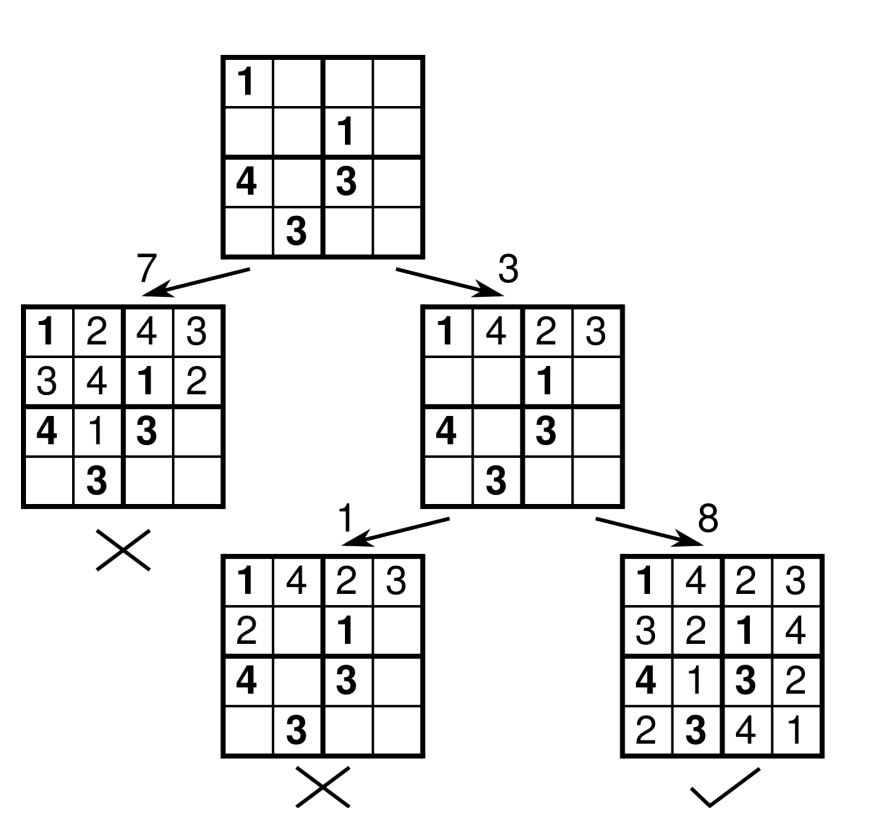
\includegraphics[scale=0.2]{./figures/backtracking.png}
		\caption{Μέρος της διαδικασίας επίλυσης ενός \(4 \times 4\) \textbf{Sudoku} με την τεχνική backtracking}
	\end{figure}
\end{frame}

\begin{frame}
	\frametitle{\el Μελέτη των επιπέδων δυσκολίας}
	\begin{itemize}
		\item \el Με την \en constraint propagation \el τεχνική χρησιμοποιούμε τη λογική για να για να βρούμε
		      την τιμή κάποιων μεταβλητών, εξετάζοντας τους περιορισμούς.
		\item \el Για κάθε μεταβλητή ορίζουμε ένα
		      σύνολο τιμών που μπορεί να λάβει χωρίς να προκαλέσει την παραβίαση κανενός περιορισμού.
		\item \el Η τεχική αυτή δεν είναι βέβαιο πως θα οδηγήσει σε λύση, αλλά σίγουρα είναι πιο αποδοτική.
		\item \el Μπορεί να συνδυαστεί με \en backtracking \el για καλύτερα αποτελέσματα.
	\end{itemize}
\end{frame}

\begin{frame}
	\frametitle{\el Μελέτη των επιπέδων δυσκολίας}
	\begin{figure}
		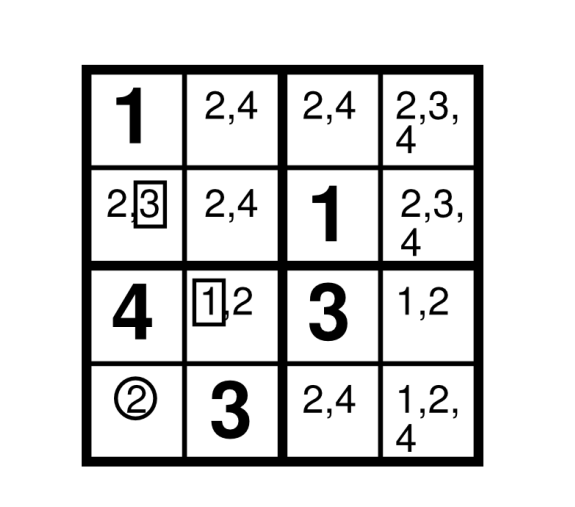
\includegraphics[scale=0.2]{./figures/propagation.png}
		\caption{Μέρος της διαδικασίας επίλυσης ενός \(4 \times 4\) \textbf{Sudoku} με την τεχνική constraint
			propagation}
	\end{figure}
\end{frame}

\begin{frame}
	\frametitle{\el Μελέτη των επιπέδων δυσκολίας}
	\begin{itemize}
		\item \el Το \en constraint propagation
		      \el είναι η τεχνική που χρησιμοποιεί ο ανθρώπινος εγκέφαλος για να επιλύσει ένα \textbf{\en Sudoku} \el παζλ.
		\item \el Συγκεκριμένα ο άνθρωπος χρησιμοποιεί δύο είδη τεχνικών:
		      \begin{itemize}
			      \item \en Naked single technique: \el όπου για ένα δεδομένο κελί του πίνακα υπάρχει μόνο μία τιμή που μπορεί να ανατεθεί, καθώς όλες οι
			            υπόλοιπες τιμές πλήττουν κάποιον περιορισμο
			      \item \en Hidden single technique: όπου για μία συγκεκριμένη γραμμή ή στήλη ή για έναν συγκεκριμένο
			            υποπίνακα του παζλ υπάρχει μόνο ένα κελί που μπορεί να φιλοξενήσει μία συγκεκριμένη τιμή.
		      \end{itemize}
	\end{itemize}
\end{frame}

\begin{frame}
	\frametitle{\el Μελέτη των επιπέδων δυσκολίας}
	\begin{itemize}
		\item \el Το πείραμα που πραγματοποιήθηκε για να συσχετίσει τη συμπεριφορά των ανθρώπων απέναντι σε παζλ, ώστε να προκύψουν συμπεράσματα για τα επίπεδα δυσκολίας τους αντλεί
		      δεδομένα από τον παγκόσμιο ιστό.
		\item \el Ως μέτρο για την εκτίμηση την δυσκολίας των ανθρώπων να λύσουν ένα παζλ \textbf{\en Sudoku} \el
		      χρησιμοποιήθηκε ο μέσος χρόνος επίλυσης.
	\end{itemize}
\end{frame}

\begin{frame}
	\frametitle{\el Μελέτη των επιπέδων δυσκολίας}
	\begin{figure}
		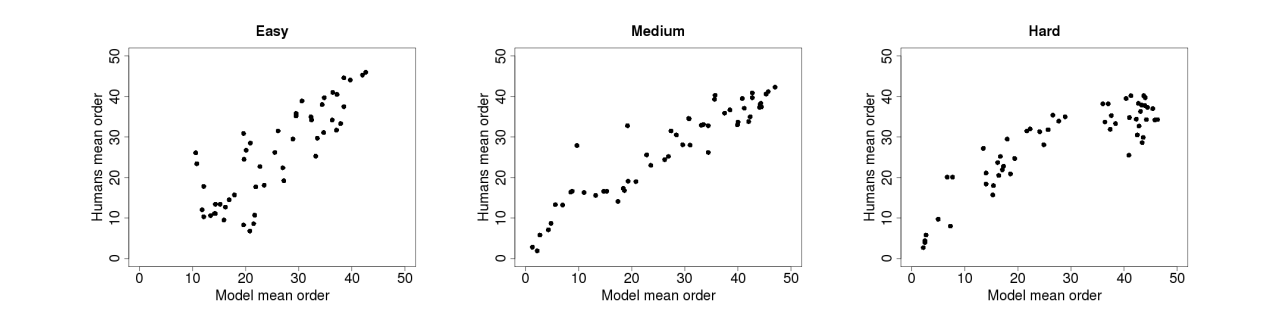
\includegraphics[scale=0.26]{./figures/results.png}
		\caption{Αποτελέσματα του πειράματος}
	\end{figure}
\end{frame}

\begin{frame}
	\frametitle{\el Στατιστική μελέτη}
	\begin{itemize}
		\item \el Παραθέτουμε στατιστική μελέτη του ζητήματος της ταξινόμησης των \textbf{\en Sudoku} \el παζλ
		      ανάλογα με το επίπεδο δυσκολίας τους, που πραγματοποιήθηκε με πραγματικά δεδομένα από το διαδίκτυο.
		\item \el Τα εν λόγω δεδομένα ήταν
		      ορθές καταχωρήσεις λυμένων παζλ από χρήστες του Διαδικτύου σε ένα καθημερινό διαγωνισμό.
		\item \el Καθημερινά συγκεντρώνονταν 2000 με 3000 καταχωρήσεις σωστά λυμένων παζλ.
	\end{itemize}
\end{frame}

\begin{frame}
	\frametitle{\el Στατιστική μελέτη}
	\begin{itemize}
		\item \el Τα επίπεδα δυσκολίας ήταν από πριν καθορισμένα και η μελέτη αυτή ήρθε να επιβεβαιώσει
		      την κατηγοριοποίηση τους σε \en ”Gentle”, ”Moderate”, ”Tough” \el και \en ”Diabolical”.
		\item \el Αφού οι άνθρωποι έλυναν κάποιο/-α παζλ έπειτα έπρεπε να δηλώσουν τον χρόνο που
		      χρειάστηκαν, για να καταφέρουν να φτάσουν στη λύση.
		\item \el Η επιλογή έγινε από συγκεκριμένα χρονικά διαστήματα,
		\item \el Παραθέτουμε τα αποτελέσματα της μελέτης.
	\end{itemize}
\end{frame}

\begin{frame}
	\frametitle{\el Στατιστική μελέτη}
	\begin{figure}
		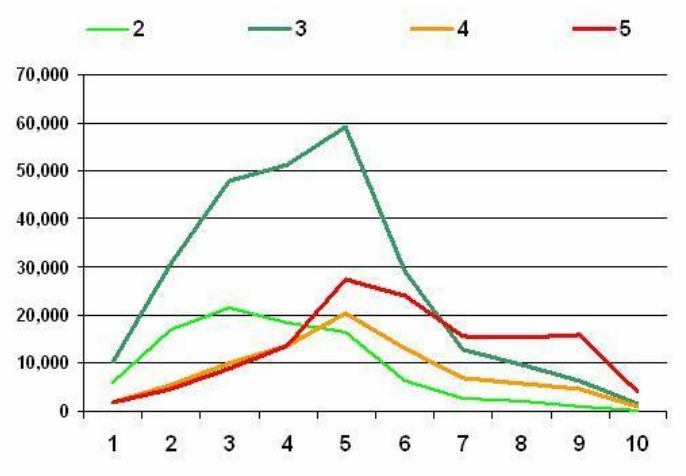
\includegraphics[scale=0.3]{./figures/stat1.png}
		\caption{Γράφημα της στατιστικής μελέτης για την ταξινόμηση των \textbf{Sudoku} ανάλογα με
			το επίπεδο δυσκολίας τους. Gentle = ανοιχτό πράσινο, Moderate = σκούρο πράσινο, Tough =
			κίτρινο, Diabolical = κόκκινο}
	\end{figure}
\end{frame}

\begin{frame}
	\frametitle{\el Στατιστική μελέτη}
	\begin{figure}
		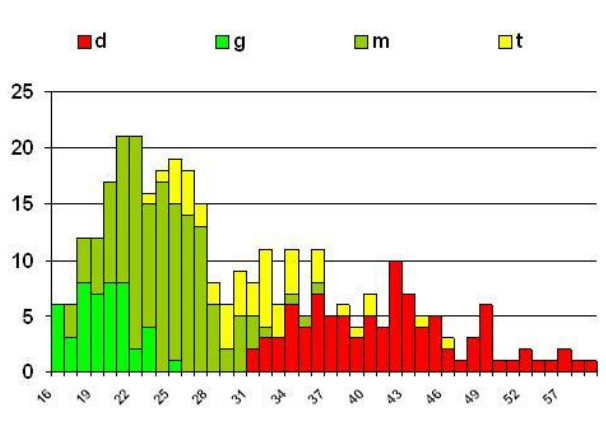
\includegraphics[scale=0.3]{./figures/stat2.png}
		\caption{Γράφημα της στατιστικής μελέτης για την ταξινόμηση των \textbf{Sudoku} ανάλογα με
			το επίπεδο δυσκολίας τους . Gentle = ανοιχτό πράσινο, Moderate = σκούρο πράσινο, Tough =
			κίτρινο, Diabolical = κόκκινο}
	\end{figure}
\end{frame}

\begin{frame}
	\frametitle{\el Στατιστική μελέτη}
	\begin{figure}
		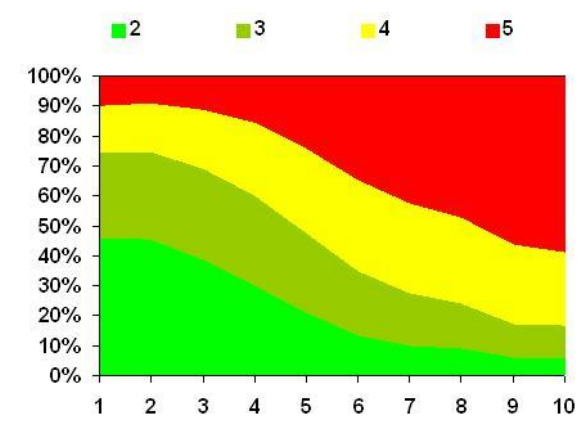
\includegraphics[scale=0.3]{./figures/stat3.png}
		\caption{Γράφημα της στατιστικής μελέτης για την ταξινόμηση των \textbf{Sudoku} ανάλογα με
			το επίπεδο δυσκολίας τους . Gentle = ανοιχτό πράσινο, Moderate = σκούρο πράσινο, Tough =
			κίτρινο, Diabolical = κόκκινο}
	\end{figure}
\end{frame}

\begin{frame}
	\frametitle{\el Δεδομένοι όροι στο παζλ}
	\begin{itemize}
		\item \el Τα συμπληρωμένα κελιά ενός παζλ καθορίζουν σημαντικά τα επίπεδα δυσκολίας	ενός παζλ.
		\item \el Το πλήθος των συμπληρωμένων κελιών, καθώς επίσης και οι θέσεις τους στον πίνακα
		      παίζουν καθοριστικό ρόλο για το πώς θα χαρακτηριστεί ένα παζλ.
		\item \el Οι παρακάτω πίνακες συνοψίζουν τη σχετική γνώση.
	\end{itemize}
\end{frame}

\begin{frame}
	\frametitle{\el Δεδομένοι όροι στο παζλ}
	\begin{center}
		\begin{tabular}{ | l | r | }
			\hline
			Επίπεδο δυσκολίας & Πλήθος δεδομένων κελιών \\

			\hline
			Πολύ εύκολο       & Περισσότερα από 46      \\
			\hline
			Εύκολο            & 36-46                   \\
			\hline
			Μέτριο            & 32-35                   \\
			\hline
			Δύσκολο           & 28-31                   \\
			\hline
			Πολύ δύσκολο      & 17-27                   \\
			\hline
		\end{tabular}
	\end{center}
\end{frame}

\begin{frame}
	\frametitle{\el Δεδομένοι όροι στο παζλ}
	\begin{center}
		\begin{tabular}{ | l | r | }
			\hline
			Επίπεδο δυσκολίας & Ελάχιστος δεδομένα κελιά ανά γραμμή/στήλη \\

			\hline
			Πολύ εύκολο       & 5                                         \\
			\hline
			Εύκολο            & 4                                         \\
			\hline
			Μέτριο            & 3                                         \\
			\hline
			Δύσκολο           & 2                                         \\
			\hline
			Πολύ δύσκολο      & 0                                         \\
			\hline
		\end{tabular}
	\end{center}
\end{frame}

\begin{frame}
	\frametitle{References}
	\begin{itemize}
		\item \textit{\en Sudoku Creation and Grading, Andrew C. Stuart, \el Φεβρουάριος 2007 - ενημερώθηκε τον Ιανουάριος 2012}
		\item \textit{\en An Exhaustive Study on different Sudoku Solving Techniques, Arnab Kumar Maji, Sunanda Jana, Sudipta Roy, Rajat Kumar Pal, International Journal of Computer Science Issues, Vol. 11, Issue 2, No 1, \el Μάρτιος 2014}
		\item \textit{\en Human Problem Solving:Sudoku Case Study, Radek Pelánek, \el Ιανουάριος 2011}
	\end{itemize}
\end{frame}

\begin{frame}
	\frametitle{References}
	\begin{itemize}
		\item \textit{"The History of Sudoku",www.sudoku.com, https://sudoku.com/how-to-play/the-history-of-sudoku/}
		\item \textit{"Howard Garns", https://en.wikipedia.org/wiki/Howard\_Garns}
		\item \textit{Binary Integer Programming and its Use for EnvelopeDetermination,
			      Vladimir Y. Lunin, Alexandre Urzhumtsev, Alexander Bockmayr}
		\item \textit{\en An Integer Programming Model for the Sudoku Problem,
			      Andrew C. Bartlett, Timothy P. Chartier, Amy N. Langville, Timothy D. Rankin, \el 3 Μάη 2008}
	\end{itemize}
\end{frame}

\begin{frame}
	\frametitle{References}
	\begin{itemize}
		\item \textit{\el Τεχνητή Νοημοσύνη Μία σύγχρονη προσέγγιση, Δεύτερη Αμερικανική έκδοση, εκδό-
			      σεις Κλειδάριθμος, \en Stuart Russell, Peter Norvig, ISBN: 960-209-873-2, \el Κεφάλαιο 5 Προβ-
			      λήματα Ικανοποίησης Περιορισμών, σελ.:179,180,181}
		\item \textit{\en The number of \(9 \times 9\) Latin squares, Discrete Mathematics, Stanley Bammel and
			      Jermome Rothstein, 1975}
		\item \textit{\en There are 6670903752021072936960 Sudoku grids, Bertram Felgenhauer and Frazer
			      Jarvis, http://www.afjarvis.staff.shef.ac.uk/sudoku/}
		\item \textit{There are 5472730538 essentially different Sudoku grids . . . and the Sudoku symme-
			      try group, Ed Russell and Frazer Jarvis, http://www.afjarvis.staff.shef.ac.uk/
			      sudoku/sudgroup.html/}
	\end{itemize}
\end{frame}

\end{document}